
\documentclass[acmtog, authorversion]{acmart}

\usepackage{booktabs} % For formal tables

\usepackage{graphicx}
\usepackage[export]{adjustbox}
\usepackage{float}
\usepackage{natbib}

% TOG prefers author-name bib system with square brackets
\citestyle{acmauthoryear}
\setcitestyle{square}


\usepackage[ruled]{algorithm2e} % For algorithms
\renewcommand{\algorithmcfname}{ALGORITHM}
\SetAlFnt{\small}
\SetAlCapFnt{\small}
\SetAlCapNameFnt{\small}
\SetAlCapHSkip{0pt}
\IncMargin{-\parindent}

% Metadata Information
\acmJournal{TOG}
\acmVolume{9}
\acmNumber{4}
\acmArticle{39}
\acmYear{2010}
\acmMonth{3}

% Copyright
%\setcopyright{acmcopyright}
%\setcopyright{acmlicensed}
%\setcopyright{rightsretained}
%\setcopyright{usgov}
\setcopyright{usgovmixed}
%\setcopyright{cagov}
%\setcopyright{cagovmixed}

% DOI
\acmDOI{0000001.0000001_2}

% Paper history
\received{February 2007}
\received{March 2009}
\received[final version]{June 2009}
\received[accepted]{July 2009}

% Document starts
\begin{document}
% Title portion
\title{A Multifrequency MAC Specially Designed for Wireless Sensor
  Network Applications}

\author{Gang Zhou}
\orcid{1234-5678-9012-3456}
\affiliation{%
  \institution{College of William and Mary}
  \streetaddress{104 Jamestown Rd}
  \city{Williamsburg}
  \state{VA}
  \postcode{23185}
  \country{USA}}
\email{gang_zhou@wm.edu}
\author{Valerie B\'eranger}
\affiliation{%
  \institution{Inria Paris-Rocquencourt}
  \city{Rocquencourt}
  \country{France}
}
\email{beranger@inria.fr}

\begin{abstract}
Multifrequency media access control has been well understood in
general wireless ad hoc networks, while in wireless sensor networks,
researchers still focus on single frequency solutions. In wireless
sensor networks, each device is typically equipped with a single
radio transceiver and applications adopt much smaller packet sizes
compared to those in general wireless ad hoc networks. Hence, the
multifrequency MAC protocols proposed for general wireless ad hoc
networks are not suitable for wireless sensor network applications,
which we further demonstrate through our simulation experiments. In
this article, we propose MMSN, which takes advantage of
multifrequency availability while, at the same time, takes into
consideration the restrictions of wireless sensor networks. Through
extensive experiments, MMSN exhibits the prominent ability to utilize
parallel transmissions among neighboring nodes. When multiple physical
frequencies are available, it also achieves increased energy
efficiency, demonstrating the ability to work against radio
interference and the tolerance to a wide range of measured time
synchronization errors.
\end{abstract}

\maketitle

\section{Introduction}

As a new technology, Wireless Sensor Networks (WSNs) has a wide
% range of applications \cite{Culler-01, Bahl-02, Akyildiz-01}, including
environment monitoring, smart buildings, medical care, industrial and
military applications. Among them, a recent trend is to develop
commercial sensor networks that require pervasive sensing of both
environment and human beings, for example, assisted living
% \cite{Akyildiz-02, Harvard-01,CROSSBOW} and smart homes
% \cite{Harvard-01, Adya-01,CROSSBOW}.
% quote
\begin{quote}
  ``For these applications, sensor devices are incorporated into human
  % cloths \cite{Natarajan-01, Zhou-06, Bahl-02, Adya-01} for monitoring
  health related information like EKG readings, fall detection, and
  voice recognition''.
\end{quote}
While collecting all these multimedia information
% \cite{Akyildiz-02} requires a high network throughput, off-the-shelf
sensor devices only provide very limited bandwidth in a single
% channel: 19.2\,Kbps in MICA2 \cite{Bahl-02} and 250\,Kbps in MICAz.

In this article, we propose MMSN, abbreviation for Multifrequency
Media access control for wireless Sensor Networks. The main
contributions of this work can be summarized as follows.
% itemize
\begin{itemize}
\item To the best of our knowledge, the MMSN protocol is the first
multifrequency MAC protocol especially designed for WSNs, in which
each device is equipped with a single radio transceiver and
the MAC layer packet size is very small.
\item Instead of using pairwise RTS/CTS frequency negotiation
% \cite{Adya-01, Culler-01, Tzamaloukas-01, Zhou-06},
we propose lightweight frequency assignments, which are good choices
for many deployed comparatively static WSNs.
\item We develop new toggle transmission and snooping techniques to
enable a single radio transceiver in a sensor device to achieve
scalable performance, avoiding the nonscalable ``one
% control channel + multiple data channels'' design \cite{Natarajan-01}.
\end{itemize}

% Head 1
\section{Feature Extraction}

Apart from the audio features that were included in the million song dataset (acousticness, tempo, instrumentalness, liveness, speechiness, valence, danceability) we also extracted the year and popularity from the Spotify API data. We also crafted 3 additional features using the modeling techniques described below.
% Head 2
\subsection{Latent Dirichlet Allocation}

We chose all playlists for which we had an overlap of at least 30 songs with our dataset. We then tokenized and removed all stop words from the lyrics of the songs from every playlist, in order for the playlists to be treated as documents and the lyrics as words in the latent Dirichlet allocation model. Latent Dirichlet allocation is a generative statistical model that posits that the lyrics from every playlist can be explained by a fixed number of unobserved groups, which would explain similarity between some playlists. In our case, we chose the number of common topics to be 3, and the process that the generative model describes is the following: \newline
For the $M$ playlists, each of length $N_{i}$ we have the following parameters and distributions:
\begin{enumerate}
  \item Probability $\theta_{i} \sim Dir(\alpha)$, where $Dir(\alpha)$ is a Dirichlet distribution with parameter $\alpha$ and $i \in {1, ..., M}$
  \item Probability $\phi_{k} \sim Dir(\beta)$, where $k \in {1,2,3}$ is the index of the topic.
  \item For each word in the lyrics from all playlists, for $i, j$, where $i \in {1, ..., M}$ and $j \in {1, ..., N_{i}}$:
     \begin{enumerate}
       \item Chose a topic $z_{i, j} \sim Multinomial(\theta_{i})$
       \item Chose a word $w_{i, j} \sim Multinomial(z_{i, j})$
     \end{enumerate}
\end{enumerate}

The probabilities that were output from the model for each of the three topics, were subsequently used as features by the final model.

% Numbered Equation
\begin{equation}
\label{eqn:01}
P(t)=\frac{b^{\frac{t+1}{T+1}}-b^{\frac{t}{T+1}}}{b-1},
\end{equation}
where $t=0,{\ldots}\,,T$, and $b$ is a number greater than $1$.


% Unnumbered Equation
\[
i=\lfloor(T+1)\log_b[\alpha(b-1)+1]\rfloor.
\]
It can be easily proven that the distribution of $i$ conforms to Equation
% (\ref{eqn:01}).

% So protocols \cite{Bahl-02, Culler-01,Zhou-06,Adya-01,
% Tzamaloukas-01, Akyildiz-01} that use RTS/CTS
controls\footnote{RTS/CTS controls are required to be implemented by
802.11-compliant devices. They can be used as an optional mechanism
to avoid Hidden Terminal Problems in the 802.11 standard and}
% protocols based on those similar to \cite{Akyildiz-01} and
for frequency negotiation and reservation are not
suitable for WSN applications, even though they exhibit good
performance in general wireless ad-hoc
networks.

% Head 3
\subsubsection{Exclusive Frequency Assignment}


In exclusive frequency assignment, nodes first exchange their IDs
among two communication hops so that each node knows its two-hop
neighbors' IDs. In the second broadcast, each node beacons all
neighbors' IDs it has collected during the first broadcast period.

% Head 4
\paragraph{Eavesdropping}

Even though the even selection scheme leads to even sharing of
available frequencies among any two-hop neighborhood, it involves a
number of two-hop broadcasts. To reduce the communication cost, we
propose a lightweight eavesdropping scheme.

\subsection{Hidden Markov Model on timbre segments}

Timbre is defined as the perceived sound quality of a musical note, sound or tone. The MSD dataset contains the time sequence of the timbre feature as a vector of 12 unbounded values centered around 0. These values represent different characteristics of the spectral
surface, ordered by degree of importance. For example, the first dimension represents the average
loudness of the segment, the second one describes brightness, the third one describes the flatness of a sound, the fourth describes sounds with a stronger attack etc. We averaged the vector features for every time segment for each song, in order to have a time series of the actual timbre of each segment.
We subsequently trained a hidden Markov model on the timbre sequence of a random sample of 5,000 songs. The model is fit using the EM algorithm which is a gradient-based optimization method and can therefore get stuck in local optima. For this reason we fit the model with various initializations and selected the highest scoring one.
The inferred optimal hidden states of the timbre segments of all songs were predicted by the model, employing the Viterbi algorithm.
For each song the optimal hidden states were averaged to provide a single description of the path followed, which was used as an additional feature by the final model.
For the training data the average value of the timbre which had a hidden value of 1 was 4.96, for hidden value of 1 they had an average value of the timbre of 13.76 and for a hidden value of 2 an average of -5.35.

% Head 2
\subsection{Sentiment analysis}

% As Algorithm~\ref{alg:one} states, for each frequency
number, each node calculates a random number (${\textit{Rnd}}_{\alpha}$) for
itself and a random number (${\textit{Rnd}}_{\beta}$) for each of its two-hop
neighbors with the same pseudorandom number generator.

% Algorithm
\begin{algorithm}[t]
\SetAlgoNoLine
\KwIn{Node $\alpha$'s ID ($ID_{\alpha}$), and node $\alpha$'s
neighbors' IDs within two communication hops.}
\KwOut{The frequency number ($FreNum_{\alpha}$) node $\alpha$ gets assigned.}
$index$ = 0; $FreNum_{\alpha}$ = -1\;
\Repeat{$FreNum_{\alpha} > -1$}{
        $Rnd_{\alpha}$ = Random($ID_{\alpha}$, $index$)\;
        $Found$ = $TRUE$\;
        \For{each node $\beta$ in $\alpha$'s two communication hops
    }{
      $Rnd_{\beta}$ = Random($ID_{\beta}$, $index$)\;
      \If{($Rnd_{\alpha} < Rnd_{\beta}$) \text{or} ($Rnd_{\alpha}$ ==
          $Rnd_{\beta}$ \text{and} $ID_{\alpha} < ID_{\beta}$)\;
      }{
        $Found$ = $FALSE$; break\;
      }
        }
     \eIf{$Found$}{
           $FreNum_{\alpha}$ = $index$\;
         }{
           $index$ ++\;
     }
      }
\caption{Frequency Number Computation}
\label{alg:one}
\end{algorithm}


Bus masters are divided into two disjoint sets, $\mathcal{M}_{RT}$
and $\mathcal{M}_{NRT}$.
% description
\begin{description}
\item[RT Masters]
$\mathcal{M}_{RT}=\{ \vec{m}_{1},\dots,\vec{m}_{n}\}$ denotes the
$n$ RT masters issuing real-time constrained requests. To model the
current request issued by an $\vec{m}_{i}$ in $\mathcal{M}_{RT}$,
three parameters---the recurrence time $(r_i)$, the service cycle
$(c_i)$, and the relative deadline $(d_i)$---are used, with their
relationships.
\item[NRT Masters]
$\mathcal{M}_{NRT}=\{ \vec{m}_{n+1},\dots,\vec{m}_{n+m}\}$ is a set
of $m$ masters issuing nonreal-time constrained requests. In our
model, each $\vec{m}_{j}$ in $\mathcal{M}_{NRT}$ needs only one
parameter, the service cycle, to model the current request it
issues.
\end{description}

Here, a question may arise, since each node has a global ID. Why
don't we just map nodes' IDs within two hops into a group of
frequency numbers and assign those numbers to all nodes within two
hops?

\section{Modeling}
\label{sec:sim}

Two different methodologies were pursued. In the first one we tried different classification algorithms both for a single playlist prediction and multiclass prediction for 26 playlists. In the second
% enumerate
\begin{enumerate}
\item Load state into microcontroller model.
\item Determine assignments needed for resolving nondeterminism.
\item For each assignment.
      \begin{enumerate}
      \item either call interrupt handler or simulate effect of next instruction, or
      \item evaluate truth values of atomic propositions.
      \end{enumerate}
\item Return resulting states.
\end{enumerate}
% Figure~\ref{fig:one} shows a typical microcontroller C program that
controls an automotive power window lift. The program is one of the
% programs used in the case study described in Section~\ref{sec:sim}.
At first sight, the programs looks like an ANSI~C program. It
contains function calls, assignments, if clauses, and while loops.
% Figure
\begin{figure}
  % \includegraphics{mouse}
  \caption{Code before preprocessing.}
  \label{fig:one}
\end{figure}

\subsection{Classification}

We first applied binary classification using a single playlist ('60s, 70s, 80s Classic Rock') as the target and randomly selecting songs that didn't belong to it as well. The training set consisted of 98 songs, while the test set included 34 songs. After standardizing the features we performed grid search on the hyper-parameters for a logistic regression and support vector machine classifier. For logistic regression the regularization strength was fine tuned employing 10-fold cross-validation, while for the support vector classifier the regularization was also optimized using grid search. The other parameters that were chosen during cross validation were the kernel (linear or exponential). For the exponential kernel $e^{-\gamma {\Vert x -x' \Vert}^{2}}$ the $\gamma$ parameter was also optimized. 


The objective of variable coalescence-based offset assignment is to find
both the coalescence scheme and the MWPC on the coalesced graph. We start
with a few definitions and lemmas for variable coalescence.

% Enunciations
\begin{definition}[Coalesced Node (C-Node)]A C-node is a set of
live ranges (webs) in the AG or IG that are coalesced. Nodes within the same
C-node cannot interfere with each other on the IG. Before any coalescing is
done, each live range is a C-node by itself.
\end{definition}

\begin{definition}[C-AG (Coalesced Access Graph)]The C-AG is the access
graph after node coalescence, which is composed of all C-nodes and C-edges.
\end{definition}

\begin{lemma}
The C-MWPC problem is NP-complete.
\end{lemma}
\begin{proof} C-MWPC can be easily reduced to the MWPC problem assuming a
coalescence graph without any edge or a fully connected interference graph.
Therefore, each C-node is an uncoalesced live range after value separation
and C-PC is equivalent to PC. A fully connected interference graph is made
possible when all live ranges interfere with each other. Thus, the C-MWPC
problem is NP-complete.
\end{proof}

\begin{lemma}[Lemma Subhead]The solution to the C-MWPC problem is no
worse than the solution to the MWPC.
\end{lemma}
\begin{proof}
Simply, any solution to the MWPC is also a solution to the
C-MWPC. But some solutions to C-MWPC may not apply to the MWPC (if any
coalescing were made).
\end{proof}

\section{Results}

Results for the two main methodologies followed are presented below.


\subsection{Classification}
The logistic regression model achieved training accuracy of 95.9\% and CV accuracy of 94.8\%. The SVC outperformed the logistic regression model, with the best model achieving training accuracy of 96.9\% and CV accuracy of 95.9\%. The best model's parameters used a linear kernel with regularization. The final test accuracy for the SVC was 94.1\%. .
The learning curve for the svm model is presented below in figure \ref{fig:learning_curve} and it shows that it generalizes well over unseen data.
\newline

The validation curve for the SVC model can be seen below in figure \ref{fig:validation_curve}, which justifies how the particular value for the regularization hyper-parameter was chosen. The cross-validation accuracy decreases as the regularization parameter C increases even though the training accuracy keeps increasing, which would indicate overfitting.

The confusion matrix for the SVC model on the test data can also be seen below in figure \ref{fig:confusion_matrix}.

The ROC curve is also plotted below in figure \ref{fig:ROC_curve} which shows an excellent area under the curve.

%figure
\begin{figure}[h]
  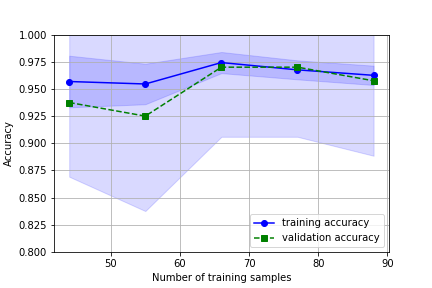
\includegraphics[width=0.5\textwidth]{learning_curve}
  \caption{Learning curve for SVC}
  \label{fig:learning_curve}
\end{figure}

%figure
\begin{figure}[h]
  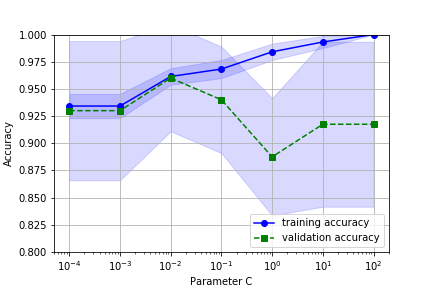
\includegraphics[width=0.5\textwidth]{validation_curve}
  \caption{Validation curve for SVC}
  \label{fig:validation_curve}
\end{figure}

%figure
\begin{figure}[h]
  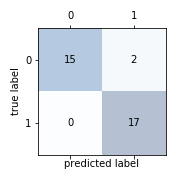
\includegraphics[width=0.33\textwidth]{confusion_matrix}
  \caption{Confusion matrix for SVC}
  \label{fig:confusion_matrix}
\end{figure}

%figure
\begin{figure}[h]
  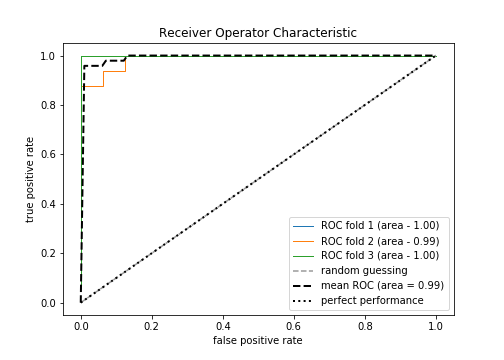
\includegraphics[width=0.5\textwidth]{ROC_curve}
  \caption{ROC curve for SVC}
  \label{fig:ROC_curve}
\end{figure}

\newpage
% Table
\begin{table}%
\caption{SVC performance on single playlist}
\label{tab:one}
\begin{minipage}{\columnwidth}
\begin{center}
\begin{tabular}{ll}
  \toprule
  Test accuracy    & 94.1\%\\
  Recall  & 100\%\\
  Precision    & 88.2\%\\
  F1-score    & 93.7\%\\
  \bottomrule
\end{tabular}
\end{center}
\bigskip\centering
\footnotesize
 \emph{Precision scores for SVC model} 
\end{minipage}
\end{table}%
\newpage
We also applied multi-class classification for 27 playlists for which we had more than 30 songs in our dataset. With this modeling technique called one-vs-all classification, one classifier is fitted for each class against all of the other classes. The training set consisted of 1265 songs, while the test set included 317 songs. Given the superior performance of the SVC model on one playlist, we optimized it in the multi-class setting using grid search and cross-validation.  



\section{Conclusions}

In this article, we develop the first multifrequency MAC protocol for
WSN applications in which each device adopts a
single radio transceiver. The different MAC design requirements for
WSNs and general wireless ad-hoc networks are
compared, and a complete WSN multifrequency MAC design (MMSN) is
put forth. During the MMSN design, we analyze and evaluate different
choices for frequency assignments and also discuss the nonuniform
back-off algorithms for the slotted media access design.

% Start of "Sample References" section

\section{Typical References in New ACM Reference Format}
% A paginated journal article \cite{Abril07}, an enumerated
% journal article \cite{Cohen07}, a reference to an entire issue \cite{JCohen96},
% a monograph (whole book) \cite{Kosiur01}, a monograph/whole book in a series (see 2a in spec. document)
% \cite{Harel79}, a divisible-book such as an anthology or compilation \cite{Editor00}
% followed by the same example, however we only output the series if the volume number is given
% \cite{Editor00a} (so Editor00a's series should NOT be present since it has no vol. no.),
% a chapter in a divisible book \cite{Spector90}, a chapter in a divisible book
% in a series \cite{Douglass98}, a multi-volume work as book \cite{Knuth97},
% an article in a proceedings (of a conference, symposium, workshop for example)
% (paginated proceedings article) \cite{Andler79}, a proceedings article
% with all possible elements \cite{Smith10}, an example of an enumerated
% proceedings article \cite{VanGundy07},
% an informally published work \cite{Harel78}, a doctoral dissertation \cite{Clarkson85},
% a master's thesis: \cite{anisi03}, an online document / world wide web
% resource \cite{Thornburg01, Ablamowicz07, Poker06}, a video game (Case 1) \cite{Obama08} and (Case 2) \cite{Novak03}
% and \cite{Lee05} and (Case 3) a patent \cite{JoeScientist001},
% work accepted for publication \cite{rous08}, 'YYYYb'-test for prolific author
% \cite{SaeediMEJ10} and \cite{SaeediJETC10}. Other cites might contain
% 'duplicate' DOI and URLs (some SIAM articles) \cite{Kirschmer:2010:AEI:1958016.1958018}.
% Boris / Barbara Beeton: multi-volume works as books
% \cite{MR781536} and \cite{MR781537}.

A couple of citations with DOIs: \cite{2004:ITE:1009386.1010128,
  Kirschmer:2010:AEI:1958016.1958018}.

% Online citations: \cite{TUGInstmem, Thornburg01, CTANacmart}.

% Appendix
\appendix
\section{Switching Times}

In this appendix, we measure the channel switching time of Micaz
% \cite{CROSSBOW} sensor devices.  In our experiments, one mote
alternatingly switches between Channels~11 and~12. Every time after
the node switches to a channel, it sends out a packet immediately and
then changes to a new channel as soon as the transmission is finished.
We measure the number of packets the test mote can send in 10 seconds,
denoted as $N_{1}$. In contrast, we also measure the same value of the
test mote without switching channels, denoted as $N_{2}$. We calculate
the channel-switching time $s$ as
\begin{displaymath}%
s=\frac{10}{N_{1}}-\frac{10}{N_{2}}.
\end{displaymath}%
By repeating the experiments 100 times, we get the average
channel-switching time of Micaz motes: 24.3\,$\mu$s.

\section{Supplementary Materials}


\begin{printonly}
  See the supplementary materials in the online version
\end{printonly}

\begin{screenonly}
\subsection{This is an Example of Appendix Subsection Head}

Channel-switching time is measured as the time length it takes for
motes to successfully switch from one channel to another. This
parameter impacts the maximum network throughput, because motes
cannot receive or send any packet during this period of time, and it
also affects the efficiency of toggle snooping in MMSN, where motes
need to sense through channels rapidly.

By repeating experiments 100 times, we get the average
channel-switching time of Micaz motes: 24.3 $\mu$s. We then conduct
the same experiments with different Micaz motes, as well as
experiments with the transmitter switching from Channel 11 to other
channels. In both scenarios, the channel-switching time does not have
obvious changes. (In our experiments, all values are in the range of
23.6 $\mu$s to 24.9 $\mu$s.)

\subsection{Appendix Subsection Head}

The primary consumer of energy in WSNs is idle listening. The key to
reduce idle listening is executing low duty-cycle on nodes. Two
primary approaches are considered in controlling duty-cycles in the
MAC layer.

\end{screenonly}

\begin{acks}

The authors would like to thank Dr. Maura Turolla of Telecom
Italia for providing specifications about the application scenario.

The work is supported by the \grantsponsor{GS501100001809}{National
  Natural Science Foundation of
  China}{http://dx.doi.org/10.13039/501100001809} under Grant
No.:~\grantnum{GS501100001809}{61273304\_a}
and~\grantnum[http://www.nnsf.cn/youngscientists]{GS501100001809}{Young
  Scientists' Support Program}.


\end{acks}

% Bibliography
\bibliographystyle{ACM-Reference-Format}
\bibliography{sample-bibliography}

\keywords{Wireless sensor networks, media access control,
multi-channel, radio interference, time synchronization}




%\input{samplebody-journals}



% Baseline: Avg distance within train set:          0.241749220274
% Avg distance of prediction to positive train set: 0.191966891286
% Avg distance of prediction to positive test set:  0.196542014849
% Avg distance of prediction to negative test set:  0.292054955012

% 19.0
% Avg distance to actual playlist: 0.231436866148

\end{document}
